
\documentclass[letterpaper,hide notes,xcolor={table,svgnames},pdftex]{beamer}
\def\showexamples{t}


%\usepackage[svgnames]{xcolor}

%% Demo talk
%\documentclass[letterpaper,notes=show]{beamer}

\usecolortheme{crane}%seahorse crane
\setbeamertemplate{navigation symbols}{}

\usetheme{MyPittsburgh}
%\usetheme{Frankfurt}

%\usepackage{tipa}

\usepackage{hyperref}
\usepackage{graphicx,xspace}
\usepackage[normalem]{ulem}

\newcommand\SF[1]{$\bigstar$\footnote{SF: #1}}

\usepackage{paratype}
\renewcommand*\familydefault{\sfdefault} %% Only if the base font of the document is to be sans serif
\usepackage[zerostyle=c]{newtxtt}
\usepackage[T1]{fontenc}

\newcounter{tmpnumSlide}
\newcounter{tmpnumNote}

\usepackage{xcolor}
\usepackage{tabu}
\definecolor{light-gray}{gray}{0.75}
\taburulecolor{light-gray}

% old question code
%\newcommand\question[1]{{$\bigstar$ \small \onlySlide{2}{#1}}}
% \newcommand\nquestion[1]{\ifdefined \presentationonly \textcircled{?} \fi \note{\par{\Large \textbf{?}} #1}}
% \newcommand\nanswer[1]{\note{\par{\Large \textbf{A}} #1}}


 \newcommand\mnote[1]{%
   \addtocounter{tmpnumSlide}{1}
   \ifdefined\showcues {~\tiny\fbox{\arabic{tmpnumSlide}}}\fi
   \note{\setlength{\parskip}{1ex}\addtocounter{tmpnumNote}{1}\textbf{\Large \arabic{tmpnumNote}:} {#1\par}}}

\newcommand\mmnote[1]{\note{\setlength{\parskip}{1ex}#1\par}}

%\newcommand\mnote[2][]{\ifdefined\handoutwithnotes {~\tiny\fbox{#1}}\fi
% \note{\setlength{\parskip}{1ex}\textbf{\Large #1:} #2\par}}

%\newcommand\mnote[2][]{{\tiny\fbox{#1}} \note{\setlength{\parskip}{1ex}\textbf{\Large #1:} #2\par}}

\newcommand\mquestion[2]{{~\color{red}\fbox{?}}\note{\setlength{\parskip}{1ex}\par{\Large \textbf{?}} #1} \note{\setlength{\parskip}{1ex}\par{\Large \textbf{A}} #2\par}\ifdefined \presentationonly \pause \fi}

\newcommand\blackboard[1]{%
\ifdefined   \showblackboard
  {#1}
  \else {\begin{center} \fbox{\colorbox{blue!30}{%
         \begin{minipage}{.95\linewidth}%
           \hspace{\stretch{1}} Some space intentionally left blank; done at the blackboard.%
         \end{minipage}}}\end{center}}%
         \fi%
}



%\newcommand\q{\tikz \node[thick,color=black,shape=circle]{?};}
%\newcommand\q{\ifdefined \presentationonly \textcircled{?} \fi}

\usepackage{listings}
\lstset{%
  keywordstyle=\bfseries,
  aboveskip=15pt,
  belowskip=15pt,
  captionpos=b,
  identifierstyle=\ttfamily,
  escapeinside={(*@}{@*)},
  stringstyle=\ttfamiliy,
  frame=lines,
  numbers=left, basicstyle=\scriptsize, numberstyle=\tiny, stepnumber=0, numbersep=2pt}

\usepackage{siunitx}
\newcommand\sius[1]{\num[group-separator = {,}]{#1}\si{\micro\second}}
\newcommand\sims[1]{\num[group-separator = {,}]{#1}\si{\milli\second}}
\newcommand\sins[1]{\num[group-separator = {,}]{#1}\si{\nano\second}}
\sisetup{group-separator = {,}, group-digits = true}

%% -------------------- tikz --------------------
\usepackage{tikz}
\usetikzlibrary{positioning}
\usetikzlibrary{arrows,backgrounds,automata,decorations.shapes,decorations.pathmorphing,decorations.markings,decorations.text}

\tikzstyle{place}=[circle,draw=blue!50,fill=blue!20,thick, inner sep=0pt,minimum size=6mm]
\tikzstyle{transition}=[rectangle,draw=black!50,fill=black!20,thick, inner sep=0pt,minimum size=4mm]

\tikzstyle{block}=[rectangle,draw=black, thick, inner sep=5pt]
\tikzstyle{bullet}=[circle,draw=black, fill=black, thin, inner sep=2pt]

\tikzstyle{pre}=[<-,shorten <=1pt,>=stealth',semithick]
\tikzstyle{post}=[->,shorten >=1pt,>=stealth',semithick]
\tikzstyle{bi}=[<->,shorten >=1pt,shorten <=1pt, >=stealth',semithick]

\tikzstyle{mut}=[-,>=stealth',semithick]

\tikzstyle{treereset}=[dashed,->, shorten >=1pt,>=stealth',thin]

\usepackage{ifmtarg}
\usepackage{xifthen}
\makeatletter
% new counter to now which frame it is within the sequence
\newcounter{multiframecounter}
% initialize buffer for previously used frame title
\gdef\lastframetitle{\textit{undefined}}
% new environment for a multi-frame
\newenvironment{multiframe}[1][]{%
\ifthenelse{\isempty{#1}}{%
% if no frame title was set via optional parameter,
% only increase sequence counter by 1
\addtocounter{multiframecounter}{1}%
}{%
% new frame title has been provided, thus
% reset sequence counter to 1 and buffer frame title for later use
\setcounter{multiframecounter}{1}%
\gdef\lastframetitle{#1}%
}%
% start conventional frame environment and
% automatically set frame title followed by sequence counter
\begin{frame}%
\frametitle{\lastframetitle~{\normalfont(\arabic{multiframecounter})}}%
}{%
\end{frame}%
}
\makeatother

\makeatletter
\newdimen\tu@tmpa%
\newdimen\ydiffl%
\newdimen\xdiffl%
\newcommand\ydiff[2]{%
    \coordinate (tmpnamea) at (#1);%
    \coordinate (tmpnameb) at (#2);%
    \pgfextracty{\tu@tmpa}{\pgfpointanchor{tmpnamea}{center}}%
    \pgfextracty{\ydiffl}{\pgfpointanchor{tmpnameb}{center}}%
    \advance\ydiffl by -\tu@tmpa%
}
\newcommand\xdiff[2]{%
    \coordinate (tmpnamea) at (#1);%
    \coordinate (tmpnameb) at (#2);%
    \pgfextractx{\tu@tmpa}{\pgfpointanchor{tmpnamea}{center}}%
    \pgfextractx{\xdiffl}{\pgfpointanchor{tmpnameb}{center}}%
    \advance\xdiffl by -\tu@tmpa%
}
\makeatother
\newcommand{\copyrightbox}[3][r]{%
\begin{tikzpicture}%
\node[inner sep=0pt,minimum size=2em](ciimage){#2};
\usefont{OT1}{phv}{n}{n}\fontsize{4}{4}\selectfont
\ydiff{ciimage.south}{ciimage.north}
\xdiff{ciimage.west}{ciimage.east}
\ifthenelse{\equal{#1}{r}}{%
\node[inner sep=0pt,right=1ex of ciimage.south east,anchor=north west,rotate=90]%
{\raggedleft\color{black!50}\parbox{\the\ydiffl}{\raggedright{}#3}};%
}{%
\ifthenelse{\equal{#1}{l}}{%
\node[inner sep=0pt,right=1ex of ciimage.south west,anchor=south west,rotate=90]%
{\raggedleft\color{black!50}\parbox{\the\ydiffl}{\raggedright{}#3}};%
}{%
\node[inner sep=0pt,below=1ex of ciimage.south west,anchor=north west]%
{\raggedleft\color{black!50}\parbox{\the\xdiffl}{\raggedright{}#3}};%
}
}
\end{tikzpicture}
}


%% --------------------

%\usepackage[excludeor]{everyhook}
%\PushPreHook{par}{\setbox0=\lastbox\llap{MUH}}\box0}

%\vspace*{\stretch{1}

%\setbox0=\lastbox \llap{\textbullet\enskip}\box0}

\setlength{\parskip}{\fill}

\newcommand\noskips{\setlength{\parskip}{1ex}}
\newcommand\doskips{\setlength{\parskip}{\fill}}

\newcommand\xx{\par\vspace*{\stretch{1}}\par}
\newcommand\xxs{\par\vspace*{2ex}\par}
\newcommand\tuple[1]{\langle #1 \rangle}
\newcommand\code[1]{{\sf \footnotesize #1}}
\newcommand\ex[1]{\uline{Example:} \ifdefined \presentationonly \pause \fi
  \ifdefined\showexamples#1\xspace\else{\uline{\hspace*{2cm}}}\fi}

\newcommand\ceil[1]{\lceil #1 \rceil}


\AtBeginSection[]
{
   \begin{frame}
       \frametitle{Outline}
       \tableofcontents[currentsection]
   \end{frame}
}



\pgfdeclarelayer{edgelayer}
\pgfdeclarelayer{nodelayer}
\pgfsetlayers{edgelayer,nodelayer,main}

\tikzstyle{none}=[inner sep=0pt]
\tikzstyle{rn}=[circle,fill=Red,draw=Black,line width=0.8 pt]
\tikzstyle{gn}=[circle,fill=Lime,draw=Black,line width=0.8 pt]
\tikzstyle{yn}=[circle,fill=Yellow,draw=Black,line width=0.8 pt]
\tikzstyle{empty}=[circle,fill=White,draw=Black]
\tikzstyle{bw} = [rectangle, draw, fill=blue!20, 
    text width=4em, text centered, rounded corners, minimum height=2em]
    
    \newcommand{\CcNote}[1]{% longname
	This work is licensed under the \textit{Creative Commons #1 3.0 License}.%
}
\newcommand{\CcImageBy}[1]{%
	\includegraphics[scale=#1]{creative_commons/cc_by_30.pdf}%
}
\newcommand{\CcImageSa}[1]{%
	\includegraphics[scale=#1]{creative_commons/cc_sa_30.pdf}%
}
\newcommand{\CcImageNc}[1]{%
	\includegraphics[scale=#1]{creative_commons/cc_nc_30.pdf}%
}
\newcommand{\CcGroupBySa}[2]{% zoom, gap
	\CcImageBy{#1}\hspace*{#2}\CcImageNc{#1}\hspace*{#2}\CcImageSa{#1}%
}
\newcommand{\CcLongnameByNcSa}{Attribution-NonCommercial-ShareAlike}


\newenvironment{changemargin}[1]{% 
  \begin{list}{}{% 
    \setlength{\topsep}{0pt}% 
    \setlength{\leftmargin}{#1}% 
    \setlength{\rightmargin}{1em}
    \setlength{\listparindent}{\parindent}% 
    \setlength{\itemindent}{\parindent}% 
    \setlength{\parsep}{\parskip}% 
  }% 
  \item[]}{\end{list}} 




\title{Lecture 22 --- ToString, Equality, Namespaces}

\author{J. Zarnett\\
\texttt{jzarnett@uwaterloo.ca}}
\institute{Department of Electrical and Computer Engineering \\
  University of Waterloo}
\date{\today}

\begin{document}

\begin{frame}
  \titlepage
  
  \begin{center}
  \small{Acknowledgments: W.D. Bishop}
  \end{center}
\end{frame}

\part{ToString}
\begin{frame}\partpage\end{frame}


\begin{frame}
\frametitle{Printing Objects}

What happens if we try writing  an object to the console with \texttt{Console.WriteLine( )}?

The class name is just printed to the console. That's not very helpful.

The system tries to convert the class to a console-printable form and that's the default behaviour. 

\end{frame}

\begin{frame}
\frametitle{The \texttt{ToString} Method}
A \texttt{ToString( )} method automatically exists for every C\# type.

The \texttt{ToString( )} method converts the value of an object to a string format in a (hopefully) meaningful way.

This method applies to both simple types and structured types.
\end{frame}

\begin{frame}
\frametitle{The \texttt{override} Keyword}
To replace the default behaviour of an existing method, like \texttt{ToString}, we need to make use of the \alert{\texttt{override}} keyword.

This is our way of indicating that we want to replace the default behaviour provided for all objects in the system.

Now we are ready to write an implementation for \texttt{Coordinates}.

\end{frame}



\begin{frame}[fragile]
\frametitle{Implementing \texttt{ToString} for \texttt{Coordinates}}

\begin{verbatim}
public override string ToString( )
{
    return "(" + x + ", " + y + ", " + z + ")";
}
\end{verbatim}

After this, whenever an object of type \texttt{Coordinates} is to be printed to the screen, it will be formatted as \texttt{(x, y, z)}. E.g., (1, 7, -5).

\end{frame}


\begin{frame}[fragile]
\frametitle{Implementing \texttt{ToString} for \texttt{Coordinates}}

The code below:

\begin{verbatim}
Coordinates c4 = new Coordinates( 1, 7, -5 );
Console.WriteLine( c4 );
\end{verbatim}

will produce as output:
\texttt{(1, 7, -5)}

\end{frame}


\begin{frame}
\frametitle{Beyond Console Printing}

The examples thus far have used \texttt{Console.WriteLine} but there are other scenarios where we might convert an object to a \texttt{string}.

\texttt{Console.WriteLine} has called \texttt{ToString} for us, but in other situations we are responsible for doing so.

The \texttt{ToString} method can be explicitly called any time we wish to convert an object to a \texttt{string}.

Example:\\
 \texttt{string positionText = "Your position:~"~+~c4.ToString();}

\end{frame}

\part{Object Equality}
\begin{frame}\partpage\end{frame}

\begin{frame}
\frametitle{Equality}


When using equality operators, \texttt{==} and \texttt{!=}, we have thus far used them on simple types like \texttt{int}; \texttt{7 == 0} evaluates to \texttt{false}.

When it comes to reference types, however, things don't always behave as we would expect.

What does it mean for two \texttt{Coordinates} objects to be equal?

\end{frame}

\begin{frame}
\frametitle{Use of the \texttt{==} Operator on Objects}
Our first instinct is to use the \texttt{==} operator.\\
\quad This results in a test of \alert{reference equality}.

This means that two objects will be considered equal if they are referring to the same object in memory.

\texttt{Coordinates c1 = new Coordinates( );}\\
\texttt{Coordinates c2 = c1; }\\
\texttt{Coordinates c3 = new Coordinates( );}

A test of \texttt{c2 == c1} will evaluate to true.\\
A test of \texttt{c1 == c3} will evaluate to false.

\end{frame}

\begin{frame}
\frametitle{Use of the \texttt{==} Operator on Objects}
Both \texttt{c1} and \texttt{c3} are initialized as (0, 0, 0).

Does this make intuitive sense when we look at this scenario?

\texttt{Coordinates c1 = new Coordinates( 1.5, -2.0, 10 );}\\
\texttt{Coordinates c2 = c1; }\\
\texttt{Coordinates c3 = new Coordinates( 1.5, -2.0, 10 );}

Even though they're both (1.5, -2.0, 10), \texttt{c1} and \texttt{c3} will not be considered equal by the \texttt{==} operator.

\end{frame}

\begin{frame}
\frametitle{Comparing Objects}
Our first approach to solving this might be to have the following statement to check if \texttt{c1} and \texttt{c3} are equal\\
\quad \texttt{c1.X == c3.X \&\& c1.Y == c3.Y \&\& c1.Z == c3.Z}

This is tedious and error-prone every time it's needed in the code (and impractical if the objects have many fields).

Apply a previous solution to this problem: make it a function!

\end{frame}

\begin{frame}
\frametitle{Comparing Objects}
You might find it logical to implement a function \texttt{Equals} for this.\\
\quad It turns out, so did the designers of C\#.

Like \texttt{ToString( )}, every object in C\# automatically has an \texttt{Equals} method that you can use to compare two objects.

Also like the default \texttt{ToString( )}, the default implementation of \texttt{Equals} is not very useful. It does the same as \texttt{==}.

\end{frame}

\begin{frame}
\frametitle{Implementing \texttt{Equals}}
We can write our own implementation for \texttt{Equals}, but must follow these rules:

\begin{itemize}
\item \texttt{x.Equals(x)} returns true
\item \texttt{x.Equals(y)} returns the same value as \texttt{y.Equals(x)}
\item \texttt{if (x.Equals(y) \&\& y.Equals(z))} returns true, then \texttt{x.Equals(z)} returns true
\item Successive invocations of \texttt{x.Equals(y)} return the same value as long as the objects referenced by \texttt{x} and \texttt{y} are not modified
\item \texttt{x.Equals(null)} returns false
\end{itemize}

Following these rules will prevent unexpected (surprising) behaviour.

\end{frame}

\begin{frame}
\frametitle{Implementing \texttt{Equals}}
The method signature for \texttt{Equals} is:\\
\quad \texttt{public override bool Equals( object obj )}

The signature compares against a general \texttt{object} and not the same class where this method is being implemented.

Recall from earlier the concept of explicit type casting: we tell the system explicitly to treat one type as another.

In this example, we need to explicitly cast \texttt{object} to \texttt{Coordinates}.

\end{frame}

\begin{frame}[fragile]
\frametitle{Implementing \texttt{Equals}}
Add the following to the \texttt{Coordinates} class:

\begin{verbatim}
public override bool Equals( object obj )
{
    if ( obj == null )
    {
        return false;
    }
    Coordinates other = (Coordinates) obj;
    
    return ( x == other.x ) 
        && ( y == other.y ) 
        && ( z == other.z );
}
\end{verbatim}

\end{frame}

\begin{frame}
\frametitle{Problem with the Previous Implementation}

There is a problem with the implementation of \texttt{Equals} on the previous slide.

What if we called \texttt{Equals} with an actual parameter that is \underline{not} an instance of \texttt{Coordinates}?

An error at this statement:\\
\quad \texttt{Coordinates other = (Coordinates) obj;}

There is, however, a way to prevent this error: the \alert{\texttt{is}} keyword.

\end{frame}

\begin{frame}
\frametitle{The \texttt{is} Keyword}

The \texttt{is} keyword gives us the ability to check if an object is an instance of a given type.

It is a binary operator that takes an object (on the left hand side) and a type name (on the right hand side), and evaluates to true or false.\\
\quad Example: \texttt{obj is Coordinates}

Apply this keyword to prevent an error in the \texttt{Equals} method.

\end{frame}

\begin{frame}[fragile]
\frametitle{Implementing \texttt{Equals} with \texttt{is}}
Add the following to the \texttt{Coordinates} class:

{\scriptsize
\begin{verbatim}
public override bool Equals( object obj )
{
    if ( obj == null )
    {
        return false;
    }
    if ( obj is Coordinates )
    {
        Coordinates other = (Coordinates) obj;
        
        return ( x == other.x ) 
            && ( y == other.y ) 
            && ( z == other.z );
    }
    else
    {
        return false;
    }
}
\end{verbatim}
}
\end{frame}

\begin{frame}
\frametitle{After Implementing \texttt{Equals}}

After implementing the \texttt{Equals} method, what happens here?

Recall this from earlier:\\
\texttt{Coordinates c1 = new Coordinates( 1.5, -2.0, 10 );}\\
\texttt{Coordinates c2 = c1; }\\
\texttt{Coordinates c3 = new Coordinates( 1.5, -2.0, 10 );}

Still \texttt{c1 == c3} will return false, because the \texttt{==} operator is still reference equality.

But \texttt{c1.Equals( c3 )} will return true.

\end{frame}

\begin{frame}
\frametitle{Another Problem with the \texttt{Equals}}
You may have noticed we are doing an \texttt{==} comparison on \texttt{double}s.\\
\quad We've previously said we should have a tolerance; not equality.

For \texttt{Coordinates}, there's another motivation to use a tolerance.


Example: if two points are close enough when drawn on the screen we may choose to consider them to be the same.

\end{frame}


\part{Namespaces}
\begin{frame}\partpage\end{frame}

\begin{frame}
\frametitle{Namespaces}
A \alert{namespace} is a collection of associated types.

Namespaces often correspond with packages, libraries, or application programming interfaces (APIs).

Namespaces permit code reuse by ensuring that types defined in one library do not conflict with those defined in another library.

Thus we could define two distinct classes called \texttt{Coordinates} and differentiate between them by putting them in different namespaces:

\texttt{Real.Coordinates} may represent $(x,y)$-coordinates;\\
\texttt{Polar.Coordinates} may represent polar $(r,\theta)$-coordinates.


\end{frame}

\begin{frame}
\frametitle{The \texttt{using} Keyword}

The \texttt{using} keyword can be used to eliminate the need for specifying the full name of a type or a function.

For example, the statement \texttt{using System;} allows a C\# program to use \texttt{System.Console.WriteLine( )} as \texttt{Console.WriteLine( )}

The scope of a \texttt{using} directive is limited to the file in which it appears; each file needs to specify its own \texttt{using} namespaces.

\end{frame}

\begin{frame}
\frametitle{C\# Type Overview}

\begin{center}
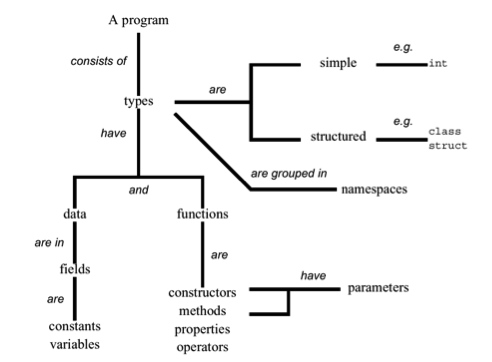
\includegraphics[width=0.8\textwidth]{images/ooterms.png}\\
{\tiny Source: J. Bishop and N. Horspool, C\# Concisely, Pearson Education Canada, 2004.}
\end{center}

\end{frame}

\end{document}

